\section*{Aufgabe 2}

\subsection*{a)}
Sei M Automat wie folgt:\\
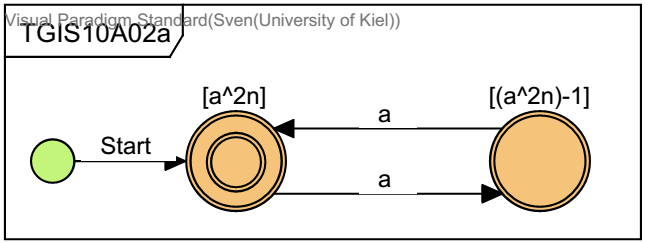
\includegraphics[width=\textwidth]{part/TGIS10A02a}
Damit ist $L(M)=L_1$

\subsection*{b)}
Sei $[a^n]$ Äquivalenzklasse zu dem Zustand den ein Automat der $L_2$ Akzeptiert bei einer Eingabe $a^n$ hat. Dann Akzeptiert nur $\widehat{\delta}([a^n], b^n c^n) $. \\
Sei $[a^{n+1}]$ Äquivalenzklasse zu dem Zustand den ein Automat der $L_2$ Akzeptiert bei einer Eingabe $a^{n+1}$ hat. Dann Akzeptiert nur $\widehat{\delta}([a^{n+1}], b^{n+1} c^{n+1}) $. Da dies für jedes $n \in N$ gilt gibt es $\infty$ viele Äquivalenzklassen.

\subsection*{c)}
Sei $|w|_a=n$ dann sei $[a^n]$ dann akzeptiert nur $\widehat{\delta}([a^{n}], b^{2n} ) $. Sei $[a^{n+1}]$ dann akzeptiert nur $\widehat{\delta}([a^{n+1}], b^{2(n+1)} ) $. Da dies für alle Äquivalenzklassen $[a^n]$ mit $n \in N$ gibt es $\infty$ viele Äquivalenzklassen.

\subsection*{d)}
Sei M Automat wie folgt:\\
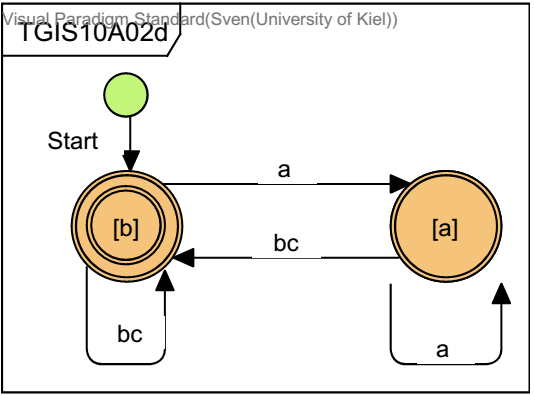
\includegraphics[width=\textwidth]{part/TGIS10A02d}
Dann ist $L(M)= L_4 $

\subsection*{e)}
Sei $[a^n]$ Äquivalenzklasse zu dem Zustand den ein Automat der $L_5$ Akzeptiert bei einer Eingabe $a^n$ hat. Dann Akzeptiert nur $\widehat{\delta}([a^n],  c a^n) $. Sei $[a^{n+1}]$ Äquivalenzklasse zu dem Zustand den ein Automat der $L_5$ Akzeptiert bei einer Eingabe $a^{n+1}$ hat. Dann Akzeptiert nur $\widehat{\delta}([a^{n+1}],  c a^{n+1}) $. Da dies für alle $n \in N$ gilt gibt es $\infty$ viele Äquivalenzklassen.